% vim: set tw=78 aw sw=2 sts=2 noet:
\documentclass{beamer}

\usepackage[english]{babel}
\usepackage[utf8x]{inputenc}
\usepackage{comment}
\usepackage{array}
\usepackage{tcolorbox}
\usepackage{verbatim}

\usepackage{subfigure}
\usepackage{graphicx}
\usepackage{float}


\usepackage[ddmmyyyy]{datetime}
\renewcommand{\dateseparator}{--}
\everymath{\displaystyle}

\mode<presentation>
{ \usetheme{Rochester} }


\title{\textbf{SA-VLSI}}
\subtitle{Sumatorul binar zecimal}
\author{Mihai Bărbulescu \\ AAC}

\begin{document}

\frame{\titlepage}

\begin{frame}{Problema}

\begin{itemize}
	\item Implementarea unui sumator BCD (Binary Coded Decimal)
	\item Tool-uri folosite:
	\begin{itemize}

		\item Icarus Verilog
		\item gtkwave
		\item Microwind 3.5
	\end{itemize}
\end{itemize}

\end{frame}

\begin{frame}{Reprezentarea numerelor în BCD}

\begin{itemize}
	\item BCD \emph{"natural"}: fiecare cifră poate fi reprezentată prin 4 biți

\begin{center}
  \begin{tabular}{| c | c | c |}
    \hline
	Decimal &	BCD Encoding \\ \hline
	0 &	0 0 0 0 \\ \hline 
	1 &	0 0 0 1 \\ \hline
	2 &	0 0 1 0 \\ \hline
	3 &	0 0 1 1 \\ \hline
	4 &	0 1 0 0\\ \hline
	5 &	0 1 0 1 \\ \hline
	6 &	0 1 1 0 \\ \hline
	7 &	0 1 1 1 \\ \hline
	8 &	1 0 0 0 \\ \hline
	9 &	1 0 0 1 \\
    \hline
  \end{tabular}
\end{center}
  \end{itemize}
\end{frame}

\begin{frame}[fragile]\frametitle{Reprezentarea numerelor în BCD (cont.)}

Calculatoarele lucrează cu octeți (8 biți). Rezultă două tipuri:

\begin{itemize}
	 \setlength{\itemsep}{1.5em}
	\item BCD neîmpachetat (ASCII). 
	\begin{itemize}  
	  \item Fiecare cifră e implementată într-un octet 
	  \item Exemplu \textbf{91} în BCD:
		\begin{verbatim}
		 9          1
		 0000 1001  0000 0001
		\end{verbatim}
	\end{itemize}
	\item BCD împachetat. 
	\begin{itemize}
	  \item Două cifre într-un octet (un număr de 2 cifre = 1 octet):
		\begin{verbatim}
		 9     1
		 1001  0001
		\end{verbatim}
	\end{itemize}
\end{itemize}
\end{frame}

\begin{frame}[fragile]\frametitle{Însumarea numerelor în BCD}

  \begin{itemize}
	\item Suma întâi în binar
	\item Apoi conversie la BCD prin adunare cu 6 când:
		\begin{itemize}
			\item Rezultatul e de 5 biți
			\item Valoarea obținută e mai mare decât 6
		\end{itemize}
  \end{itemize}

\begin{verbatim}
1001 + 1000 = 10001
  9  +    8 =    17

10001 + 0110 = 00010111 => 0001 0111
17    +    6 =       23       1    7
\end{verbatim}


\end{frame}

\begin{frame}{Schema bloc}

\begin{figure}[H]
	\centering
	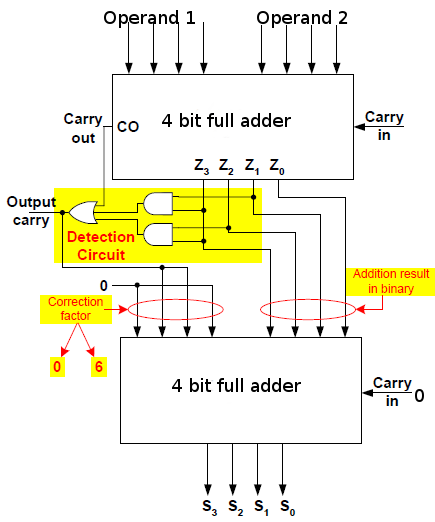
\includegraphics[scale=0.35]{../img/1digitBCDadder.png}
\end{figure}

\end{frame}

\begin{frame}{Implementare full adder 1 bit}

\begin{figure}[H]
	\centering
	\includegraphics[scale=0.75]{../img/fullAdder.jpg}
\end{figure}

\end{frame}

\begin{frame}{Implementare full adder 4 bit}

\begin{figure}[H]
	\centering
	\includegraphics[scale=0.33]{../img/4bitfa.png}
\end{figure}

\end{frame}

\begin{frame}{Full adder - simulare}

\begin{figure}[H]
	\centering
	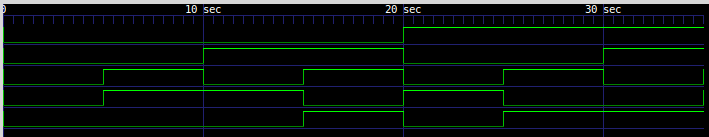
\includegraphics[scale=0.4]{fulladder1bit.png}
	\caption{Simulare Full Adder 1 bit}
\end{figure}

\begin{figure}[H]
	\centering
	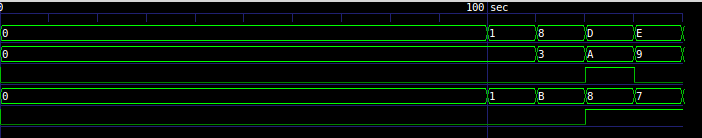
\includegraphics[scale=0.4]{fa4bit.png}
	\caption{Simulare Full Adder 4 bit}
\end{figure}

\end{frame}

\begin{frame}{BCD Adder 1 digit}

\begin{figure}[H]
	\centering
	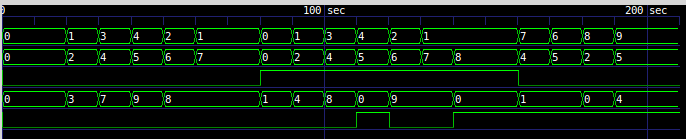
\includegraphics[scale=0.45]{bcd1digi.png}
	\caption{Simulare BCD Adder 1 digit}
\end{figure}

\end{frame}

\begin{frame}{Generalizare: BCD 2 digit - Schema bloc}

\begin{figure}[H]
	\centering
	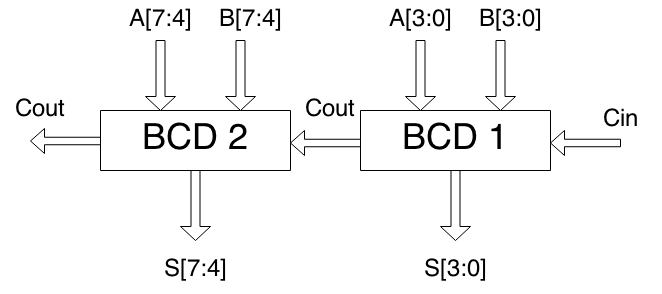
\includegraphics[scale=0.45]{../img/2digitBCD.png}
\end{figure}

\end{frame}


\begin{frame}[fragile]\frametitle{Generalizare: BCD M digit (M parametrizabil)}

\begin{verbatim}
module bcd_adder_Ndigit(sum,cout,x,y,cin);
	
    parameter M = 3; //number of digits
    parameter N = 4 * M; //number of bits required. Must be 4 * M

	input [N-1:0] x,y;
	input cin;
	
	output [N-1:0] sum;
	output cout;

	wire [N:0] carry_temp;
    assign carry_temp[0] = cin;

\end{verbatim}

\end{frame}

\begin{frame}[fragile]\frametitle{Generalizare: BCD M digit (M parametrizabil)}

\begin{verbatim}
    generate
        genvar i;

    	  for(i = 0; i < N; i=i+4) begin
            bcd_adder bcdadd(sum[i+3:i], carry_temp[i+4],
							x[i+3:i], y[i+3:i],
							carry_temp[i]);    
        end

    endgenerate

   assign cout = carry_temp[N];

endmodule
\end{verbatim}

\end{frame}



\begin{frame}{Îmbunătățiri}

\begin{itemize}
\item TODO
\end{itemize}
\end{frame}


\begin{frame}{Cuvinte cheie}
\begin{columns}[T] % align columns
\begin{column}{.48\textwidth}


\begin{itemize}
\setlength\itemsep{1.5em}
  \item constante zecimale codificate binar (BCD)
  \item sumator
  \item verilog
  \item octeți
\end{itemize}

\end{column}%
\hfill%
\begin{column}{.48\textwidth}
\begin{itemize}
\setlength\itemsep{1.5em}
  \item gtkwave
  \item porți logice elementare
\end{itemize}

\end{column}%
\end{columns}
\end{frame}

\begin{frame}{Întrebări}
  \begin{center}
    \bfseries
    \Huge
    ?
  \end{center}
\end{frame}

\end{document}
